\section{TRANSIENT THERMAL ANALYSIS}
\normalsize{Transient thermal analysis is carried out to assess the different time duration at which:
\begin{itemize}
    \item the maximum operational temperature of the parts is exceeded.
    \item the thermal equilibrium is atteigned.
    \item the effect of high temperature gradient on the evolution of the part temperature.
\end{itemize}
Those points will help us better understand the thermal bahevior of the tile and maybe allow to set time constraints on pulse duration to avoid damaging the assembly.}
\subsection{Analysis for HE1 to HE4 pulse duration}
\normalsize{During the operational life \acrshort{W7-X}, the device will be used in different operational phases. Each operational phase has different and specific operational parameters such as the plasma pulse duration \cite{Lorenz2020}. The plasma pulse duration are called $HE$ and have a number to caracterize them. There are 5 different pulse length (noted $HE1$ to $HE4$).}
\\
\begin{figure}[h!]
    \label{fig_5_12} 
    \centering
    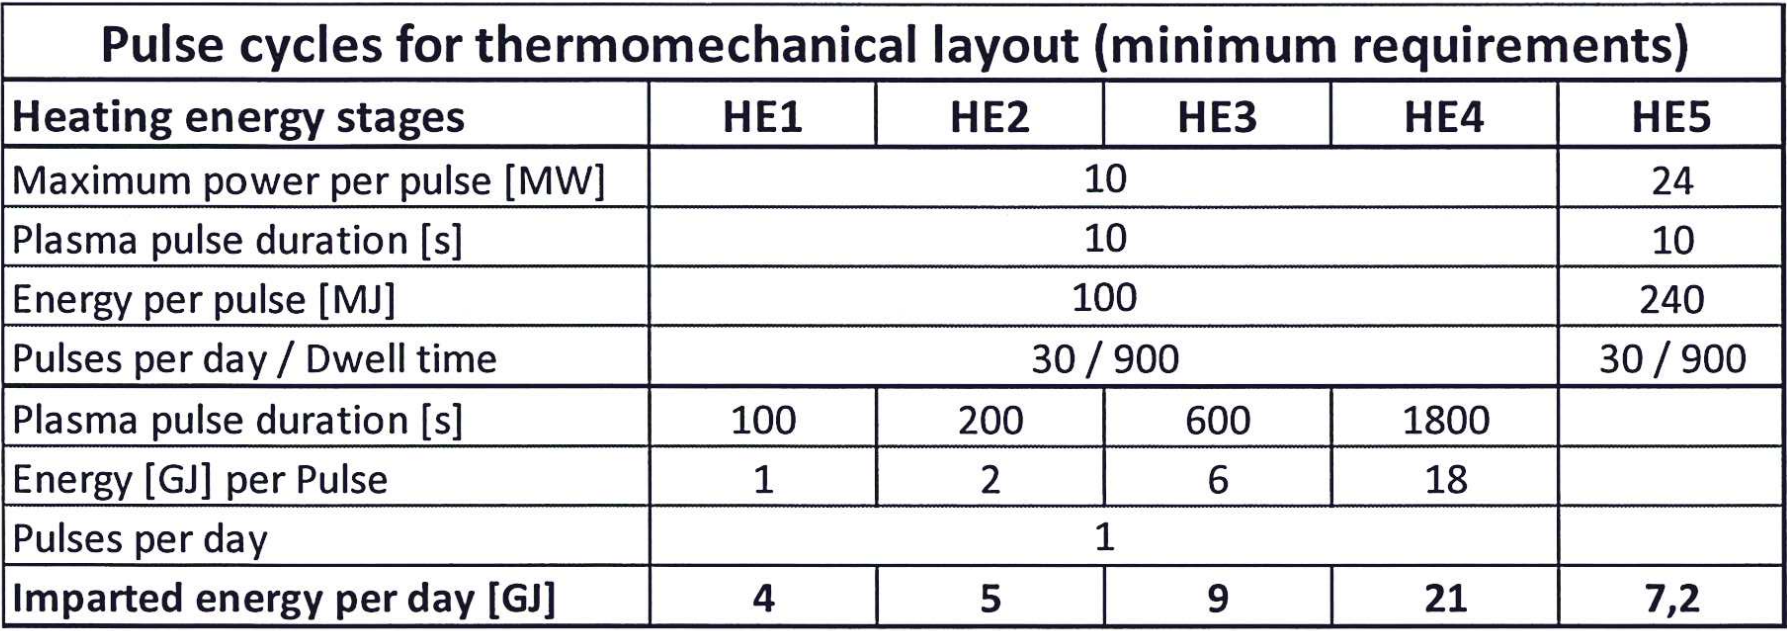
\includegraphics[width=1\textwidth]{figures/pulselengthtable.png}
    \caption{\it Table of the pulse durations \cite{Lorenz2020}}
\end{figure}
\\
\normalsize{\indent For \acrshort{OP2}, the next operation phase of \acrshort{W7-X}, the nest pulse duration is {\bfseries $HE2$} (in an ideal case, the parts of the tile assembly should not exceed their maximum temperature). The tile assembly will simulated for all cases except $HE5$. The pulse is modelled by a step function and the boundary conditions are the same as the one for the static thermal analysis \ref{Load case influence on thermal behavior}.}
\\
\break
\normalsize{\indent It is also important to calculate a minimum timestep to avoid calculation errors. For this, it is necessary to set a Fourier number and use its definition to calculate the minimum timestep. We set the Fourier number $Fo$ to be 10 (enough time has passed to the tile to reach equilibirum temperature). It is important to note that this number is a placeholder and is assumed to be that value.}
\\
\break
\normalsize{\indent The solver is set for 5 loadsteps:
\begin{itemize}
    \item Loadstep 1 is the initial pulse start with small timesteps.
    \item Loadstep 2 is the HE1 pulse (100s).
    \item Loadstep 3 is the HE2 pulse (200s).
    \item Loadstep 4 is the HE3 pulse (600s).
    \item Loadstep 5 is the HE4 pulse (1800s).
\end{itemize}
With that in mind, it is possible to run the calculations. The way the results are calculated is by dividing the maximum temperature of the parts by their respective maximum operational temperature. This allows to measure the distance between the maximum temperature and the operational temperature. When the maximum temperature exceeds the operational temperature, it is also possible to now when (when the ratio is equal to 1) and how much.}
\\
\begin{figure}[!ht]
    \label{fig_5_13} 
    \centering
    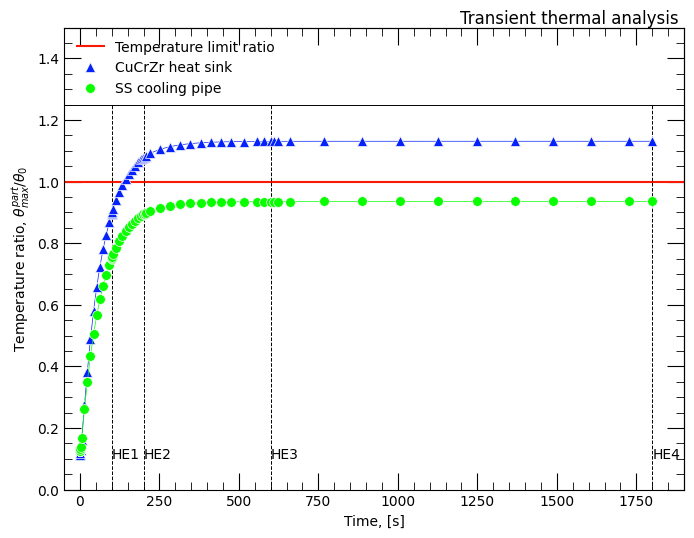
\includegraphics[width=1\textwidth]{figures/AllHEPulsesTRatio.png}
    \caption{\it Evolution of the temperature ratio $\frac{\theta^{part}_{max}}{\theta_0}$ in function of time (with echelon at all HE pulse steps). Calculation done for the load case : Plasma heat load + \acrshort{ECRH} axisymmetric heat load.}
\end{figure}
\\
\normalsize{\indent  It is nontheless important to keep in mind that technically, the maximum temperature of the heat sink change with respect to the stress, this analysis being entirely thermal doesn't take this into account. It is now possible to conclude on several different points
\begin{itemize}
    \item The \acrshort{CuCrZr} heat sink atteigns and exceeds maximum operational temperature {\bfseries 143 \unit{s} } after pulse start.
    \item For $HE2$, the temperature of the heat sink is exceed by about 1.08 $\times$ the max. allowable temperature (450 \unit{\si{\degree}C}).
    \item Quasi-steady-state is reached about 250 \unit{s} after pulse start.
    \item {\bfseries The heat sink doesn't respect specifications if max. \acrshort{CuCrZr} operational temperature is 450 \unit{\si{\degree}C}}.
\end{itemize}
}
\subsection{Analysis for HE1 pulse length and cooldown}
\normalsize{Because of the nature of heat transfer, for short duration, high heat fluxes, the heat wave travels at a certain speed, causing temperature increase {\bfseries after} shutdown of the heat load. This latent heat diffusion effect was seen by Vojtěch Smolík and the \acrshort{NBI} dump tile. The heat load was 10 \unit{MWm^{-2}} during a fraction of a second. At this heat flux, the heat wave would heat the heat sink even after shutdown of the \acrshort{NBI}. To assess this effect of latent heating, the \acrshort{ECRH} reflector tile will be exposed to $HE1$ pulse duration (100 \unit{s}) with 300 \unit{s} of cooldown. This transient analysis will help assess the magnitude of the latent heating phenomena.}
\begin{figure}[!ht]
    \label{fig_5_13} 
    \centering
    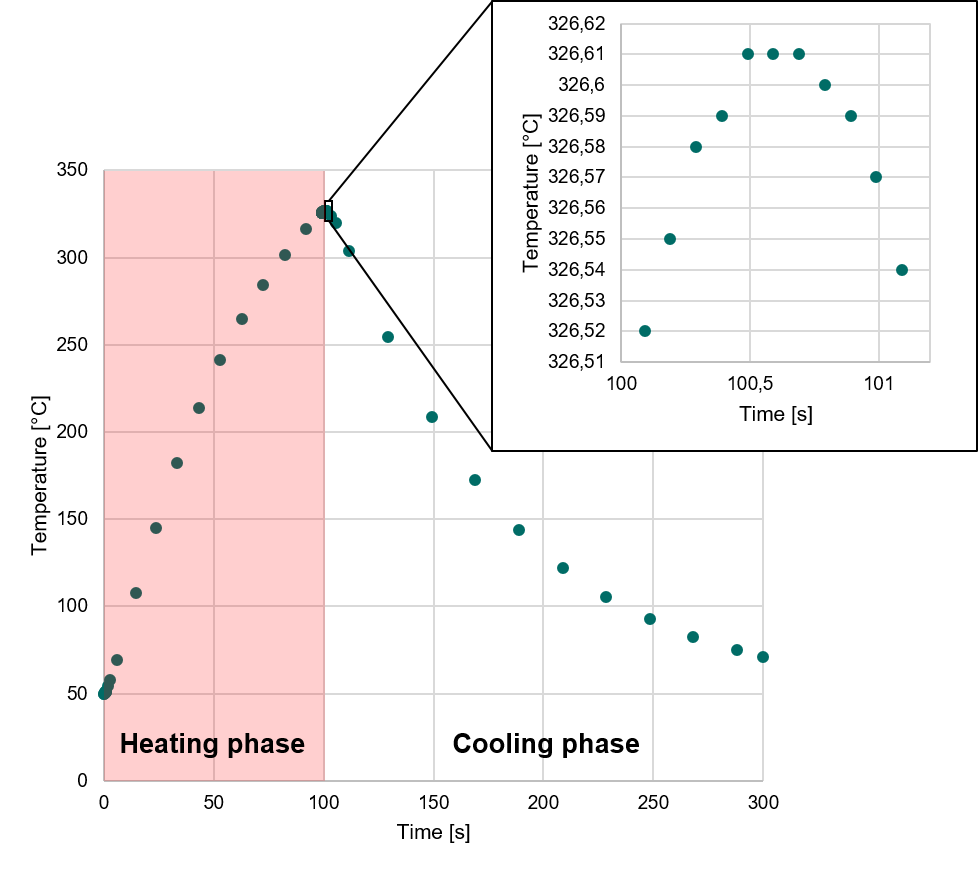
\includegraphics[width=.9\textwidth]{figures/HEATSINKLatentHeatingII.png}
    \caption{\it Evolution of the maximum temperature of the \acrshort{CuCrZr} heat sink for 100 \unit{s} pulse and 300 \unit{s} cooldown.}
\end{figure}
\\
\normalsize{\indent The results show that the latent heat diffusion phenomenon is negligeable with a temperature increase of approximately 0,1 \unit{\si{\degree}C} over the span of about 0,5 \unit{s}. This temperature increase is very small and doesn't greatly affect the general behavior of the tile assembly.}